\begin{document}

\tableofcontents
\pagebreak

%%%%%%%%%%%%%%%%%%%%%%%%%%%%%%%%%%%%%%%%%%%%%%%%%%%%%%%%%%%%%%%%%%%%%%%%%%%%%%%%%%%%%%%%%



\section{La biblioteca OpenCV.}

OpenCV (Open Source Computer Vision Library) se lanza bajo licencia BSD y, por lo tanto, es gratuito tanto para uso académico como comercial. Tiene interfaces C ++, Python y Java y es compatible con Windows, Linux, Mac OS, iOS y Android. OpenCV fue diseñado para la eficiencia computacional y con un fuerte enfoque en aplicaciones en tiempo real. Escrito en C / C ++ optimizado, la biblioteca puede aprovechar el procesamiento de múltiples núcleos. Habilitado con OpenCL, puede aprovechar la aceleración de hardware de la plataforma informática heterogénea subyacente.

Adoptado en todo el mundo, OpenCV tiene más de 47 mil personas de usuarios y una cantidad estimada de descargas que supera los 14 millones. El uso va desde el arte interactivo hasta la inspección de minas, la costura de mapas en la web o la robótica avanzada. \cite{OpenCVWebSite}


OpenCV, es una biblioteca informática de código abierto desarrollado originalmente por la visión de Intel . Es gratuito para uso comercial y la investigación bajo un licencia BSD. La biblioteca es multiplataforma y funciona en Mac OSX, Windows y Linux. Se centra principalmente hacia procesamiento imagen tiempo real como tal si encuentra Intel Integrated Performance Primitives sobre el sistema, utilizará estas rutinas optimizado comerciales a acelerarse.
Diseño del proyecto

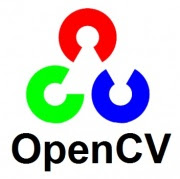
\includegraphics[width=\textwidth]{unnamed (9).jpg}

OpenCV.

Lanzado oficialmente en 1999, el proyecto fue inicialmente OpenCV iniciativa de investigación del Intel para avanzar en la CPU aplicaciones de uso intensivo, que forma parte de una serie de proyectos, entre ellos en tiempo real el trazado de rayos y las paredes de visualización 3D. Los principales contribuyentes al proyecto incluye equipo de Intel la biblioteca de rendimiento. En los primeros días de OpenCV, los objetivos del proyecto se describe como:
Avanzar en la investigación, proporcionando la visión no sólo libre, sino también el código optimizado para las infraestructuras básicas de la visión.
Difundir el conocimiento de la visión de aportar una infraestructura común que los desarrolladores pueden construir, para que el código sería más fácil lectura e intransferible.
Promover la visión basada en aplicaciones comerciales, haciendo portátiles, rendimiento optimizado de código disponible de forma gratuita con una licencia que no requiere ser abierto o gratuitas.

Historia.

Desde que apareció su primera versión alfa en el mes de enero de 1999, se ha utilizado en infinidad de aplicaciones. Desde sistemas de seguridad con detección de movimiento, hasta aplicativos de control de procesos donde se requiere reconocimiento de objetos. Esto se debe a que su publicación se da bajo licencia BSD, que permite que sea usada libremente para propósitos comerciales y de investigación con las condiciones en ella expresadas.
OpenCV es multiplataforma, existiendo versiones para GNU/Linux, Mac OSX y Windows. Contiene más de 500 funciones que abarcan una gran gama de áreas en el proceso de visión, como reconocimiento de objetos (reconocimientos facial), calibración de cámaras, visión estéreo y visión robótica.
El proyecto pretende proporcionar un entorno de desarrollo fácil de utilizar y altamente eficiente. Esto se ha logrado, realizando su programación en código C y C++ optimizados, aprovechando además las capacidades que proveen los procesadores multi núcleo. OpenCV puede además utilizar el sistema de primitivas de rendimiento integradas de Intel, un conjunto de rutinas de bajo nivel específicas para procesadores Intel (IPP).

Funciones.

Captura en tiempo real.
Importación de archivos de vídeo.
El tratamiento básico de imágenes (brillo, contraste, umbral).
Detección de objetos (cara, cuerpo).
Blob detección.

Aplicaciones.

OpenCV ha sido usado en el sistema de visión del vehículo no tripulado Stanley de la Universidad de Stanford, el ganador en el año 2005 del Gran desafío DARPA
OpenCV se usa en sistemas de vigilancia de vídeo
OpenCV es la clave en el programa Swistrack, una herramienta de seguimiento distribuida

Lenguaje de programación.

La biblioteca fue originalmente escrita en C y esta interfaz C hace OpenCV portátil para algunas plataformas específicas,tales como procesadores de señal digital.
OpenCV incluye tanto la interfaz de C tradicionales, así como una nueva interfaz C++, que busca reducir el número de líneas de código necesarias al código de la funcionalidad de la visión, así como reducir los errores comunes de programación, tales como la memoria fugas que pueden surgir al utilizar OpenCV en la mayoría de los nuevos desarrollos y algoritmos OpenCV C.
Se desarrollan en el interfaz C++, es mucho más difícil para las envolturas en otras lenguas de código C++ en lugar de código en C. \cite{SourceForceWebSite} \cite{UbaaWebSite} \cite{YahooWebSite}

\end{document}